% !TEX root=../main.tex
\section{Introduction}\label{sec:introduction}

%Faults may bring economic or even health losses.
Fault diagnosis is critical in many domains, \textit{e.g.}, machinery maintenance~\cite{Yi:2021}, petroleum refining~\cite{Dhaou:2021}, and cloud system operations~\cite{Pool:2020,Zhang:2021},  which is an active research topic in the SIGKDD community.
In this work, we focus on root cause analysis (RCA) in online service systems (OSS), such as social networks, online shopping, search engine, \textit{etc}.
We adopt the terminology in \cite{Notaro:2021}, denoting a \textit{failure} as the undesired deviation in service delivery and a \textit{fault} as the cause of the failure.

With the expansion of system scale and the rise of microservice applications, OSS are more and more complex.
As a result, operators rely on monitoring data to understand what happens in the system~\cite{Beyer:2016}.
Common monitoring data include metrics, semi-structural logs, and invocation traces.
As the most widely available data, metrics are usually in the form of time series sampled at a constant frequency, \textit{e.g.}, once per minute.
Several metrics are the measures of the overall system health status, named the \textit{service level indicator}s (SLI), \textit{e.g.}, the average response time of an online service.
Once an SLI violates the pre-defined service level objective (\textit{i.e.}, a failure occurs), operators will mitigate the failure as soon as possible to prevent further damage.
As a single fault may propagate in the system~\cite{Gertler:1998} with multiple metrics being abnormal during a failure (named \textit{anomaly storm}~\cite{Zhao:2020}), RCA (recognizing a small set of \textit{root cause indicators}) of the underlying fault can save much time for failure mitigation.
% \wenchi{It's helpful to give examples of some common indicators, such as CPU utilization, service average response time and so on...}

With the rising emphasis on explainability in many domains, \textit{causal inference}~\cite{Yao:2021} has attracted much attention in the literature.
Though causal inference is promising, causal inference-based RCA is little studied, except Sage~\cite{Gan:2021} with counterfactual analysis.
In this paper, we novelly map a fault in OSS as an intervention~\cite{Pearl:2009} in causal inference.
From this point of view, we name a new causal inference task as \textit{intervention recognition} (IR), \textit{i.e.}, finding the underlying intervention based on the observations (Definition~\ref{def:intervention-recognition}).
Hence, we formulate RCA in OSS as an IR task.

The first challenge of the new IR task is the lack of a solution.
Though Sage~\cite{Gan:2021} conducts RCA via counterfactual analysis, the design of Sage implies an implicit assumption, \textit{i.e.}, there is no intervention to the system.
Hence, Sage is not a solution to the IR task.
Based on the definition of IR, we find that the probability distribution of an intervened variable changes conditioned on parents in the Causal Bayesian Network (CBN). This \nameref{thm:rc-criterion} points out an explainable way to conduct RCA.

The second challenge is to obtain the CBN for causal inference in OSS.
Many works have been done for \textit{causal discovery}~\cite{Guo:2020} from observational data.
MicroHECL~\cite{Liu:2021} and Sage~\cite{Gan:2021} utilize the call graph in OSS, which operators are familiar with.
However, these two works consider a few metrics, \textit{e.g.}, the latency between services.
We construct the CBN among metrics with the domain knowledge of system architecture, combined with a set of intuitive assumptions, handling more kinds of metrics than MicroHECL~\cite{Liu:2021} and Sage~\cite{Gan:2021}.

Thirdly, observational knowledge is incomplete, indicating the difficulty of reaching interventional knowledge even with a perfect CBN.
For example, \figref{fig:ood} shows the joint distribution of the \textit{Average Active Session} (AAS) and the number of \textit{log file sync} waiting events around a high AAS failure of an Oracle database instance.
% Observed data before the failure are in the bottom-left corner of the figure, while the data after the failure distribute towards the far top-right corner.
% The lack of overlap blocks the comparison between these two distributions for intervention recognition.
Observed data before the failure are in the bottom-left corner of the figure.
Hence, how AAS normally distributes is missing when ``\#(log file sync)'' is larger than 1,000, where the data after the failure distribute.
The lack of overlap between the two distributions around the failure blocks recognizing intervention, if any, in AAS.
To address this challenge, we transform distribution comparison as point-wise hypothesis testing via the regression technique.
Moreover, a descendant adjustment technique is proposed to alleviate the bias introduced by a poor understanding of the system's normal status in the hypothesis testing.

\begin{figure}[t]
	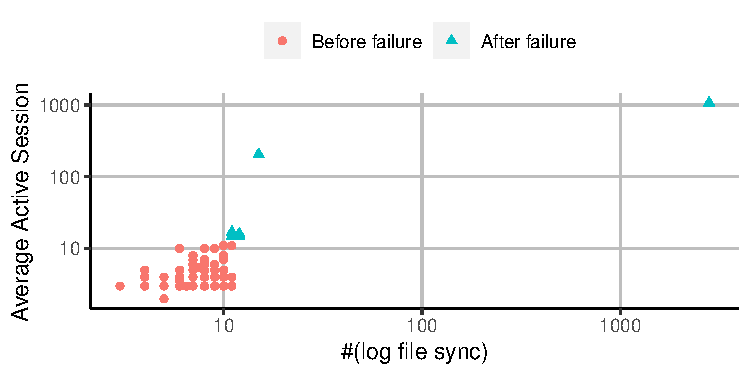
\includegraphics[width=0.85\columnwidth]{img/ood}
	\caption{Joint distribution of the \textit{Average Active Session} (an SLI of the Oracle database) and the number of \textit{log file sync} waiting events within 2 hours. Each data point represents the two metrics' values at the same timestamp.}\label{fig:ood}
	\Description{
		This figure is a scatter plot between the number of \textit{log file sync} waiting events (x-Axis) and the \textit{Average Active Session} (AAS for y-Axis) around a high AAS failure.
		Observed data before the failure are in the bottom-left corner of the figure, while the data after the failure distribute towards the far top-right corner.
	}
\end{figure}

We implement the proposed Causal Inference-based Root Cause Analysis (CIRCA).
CIRCA outperforms baseline methods in our simulation study, illustrating its theoretical reliability.
We further evaluate CIRCA with a real-world dataset.
CIRCA improves the recall of the top-1 recommendation by 25\% over the best baseline method, which shows the practical potential of our approach.
The contributions of this work are summarized as follows.

\begin{itemize}
	\item For the first time in the literature, we formulate the RCA problem in OSS as a new causal inference task named \textit{intervention recognition} (Definition~\ref{def:intervention-recognition}).
	Utilizing the advance of causal inference, we find a practical criterion to locate the root cause (\thmref{thm:rc-criterion}).
% 	Utilizing the advance of causal inference, we find a criterion to locate the root cause (\thmref{thm:rc-criterion}), which is proven to be practical.
	\item We propose Causal Inference-based Root Cause Analysis (CIRCA) for OSS.
	We propose a practical guideline to construct the CBN with the knowledge of system architecture.
	Two more techniques, namely regression-based hypothesis testing and descendant adjustment, are proposed to infer root cause metrics in the graph.
	\item CIRCA is evaluated with both simulation and real-world datasets.
	The simulation study illustrates CIRCA's theoretical reliability, while the real-world dataset shows CIRCA's practical value over baseline methods.
\end{itemize}

% The rest of this paper is organized as follows.
% In the next section, we first provide preliminary material, followed by the formal definitions of IR and RCA discussed in this work.
% \secref{sec:rc-criterion} introduces our analysis framework, while \secref{sec:methodology} describes the design of CIRCA.
% In \secref{sec:experiments}, We evaluate different methods on both simulation and real-world datasets.
% Finally, we introduce related works in \secref{sec:related-work} and conclude in \secref{sec:conclusion}.
